\section{The Tiered Cascade Hybrid (TCH)}
\label{sec:tch}

\begin{figure}[t]
\centering
\begin{minipage}{0.93\linewidth}
\small
\begin{verbatim}
                INPUT:  one 5-minute telemetry window
                        (logs, traces, metrics, k8s events,
                         94 derived numeric features,
                         visible Jira memory)

                  +----------------------+
                  |  Six pre-computed    |
                  |    pipelines run     |
                  |  (HGB, BiEncoder,    |
                  |   HRRF-rule, HRRF-LLM,
                  |   logseq2vec, KG-ret)|
                  +----------+-----------+
                             |
       +---------------------+----------------------+----------------+
       |                     |                      |                |
       v                     v                      v                v
+-------------+    +----------------------+   +----------+   +-----------------+
|     L1      |    |          L2          |   |    L3    |   |       L4        |
|  TRIAGE     |    |     RETRIEVAL        |   | NOVELTY  |   |  COMPOSITION    |
|             |    |                      |   |          |   |                 |
| LogReg over |    |  POSITION 1:         |   | OR of:   |   | pack into:      |
| 6 triage    |    |   BiEncoder top-3 +  |   |  - agent | -->|  triage_score  |
| scores      |    |   overlap rerank     |   |  - free  |   |  matched_ids[5]|
| (5-fold CV) |    |   (votes from        |   |  - learned |  |  is_novel      |
|             |    |    HRRF, logseq2vec) |   |    (G7)  |   |                 |
| threshold   |    |  POSITIONS 2..5:     |   |          |   |                 |
| tau = 0.5   |    |   RRF over 4 retrs   |   |          |   |                 |
|             |    |   (k = 60, top-10)   |   |          |   |                 |
+-------------+    +----------------------+   +----------+   +-----------------+

  OPTIONAL  +---------------------------+
  LLM PATH  | DiagnosisAgent (Qwen 35B) |
  (on all   | 3 stages: hypothesize ->  |---feeds L3 with is_novel
   1008 wins |  retrieve -> verify       |
   after G4)|  (~30 sec / window)       |
            +---------------------------+
\end{verbatim}
\end{minipage}
\caption{The TCH cascade. Six pre-computed pipelines feed four layers: L1 triage gating, L2 retrieval fusion, L3 novelty detection, L4 output composition. The agent (right) is the only inference-time LLM and feeds only the L3 novelty channel.}
\label{fig:tch-arch}
\end{figure}

\subsection{Design principle: cheap-and-broad first, expensive-and-narrow last}

The cascade has four layers, each consuming the previous layer's output plus the raw per-pipeline predictions cached upstream. The ordering is governed by per-call cost: \hgb{} (1~ms) gates the cheap triage; classical RRF (a few hundred microseconds) does fusion; the LLM agent (30 s) runs only on the hardest windows; final composition is a dict assembly.

\begin{table}[h]
\centering
\caption{The four layers and their roles.}
\label{tab:layers}
\small
\begin{tabular}{lll}
\toprule
Layer & Job & Output \\
\midrule
L1 (Triage gate) & Decide if window is real or noise & \texttt{triage\_score} $\in [0,1]$ \\
L2 (Retrieval fusion) & Produce ranked top-5 past tickets & \texttt{matched\_issue\_ids[5]} \\
L3 (Novelty check) & Flag windows with no good past match & \texttt{is\_novel} $\in \{$T, F$\}$ \\
L4 (Output composition) & Pack into the final result object & \texttt{\{score, top-5, novel\}} \\
\bottomrule
\end{tabular}
\end{table}

\subsection{L1: triage gate}

A class-balanced logistic regression stacker takes the six pipeline-level triage scores as features and produces a single calibrated probability:

\[
z = \sum_{i=1}^{6} w_i x_i + b, \qquad
P(\text{ticket\_worthy}) = \sigma(z) = \frac{1}{1 + e^{-z}}
\]

The stacker is trained on the train+val split via 5-fold \texttt{StratifiedKFold} cross-validation (\texttt{random\_state}=42, \texttt{class\_weight=balanced}). This produces honest out-of-fold predictions: every training window is scored by a model that never saw it during fit. The five fold models are then averaged for inference on test.

The learned coefficients are dominated by \hgb{} (Table~\ref{tab:l1-coefs} and Fig.~\ref{fig:l1-coefs}):

\begin{figure}[h]
\centering
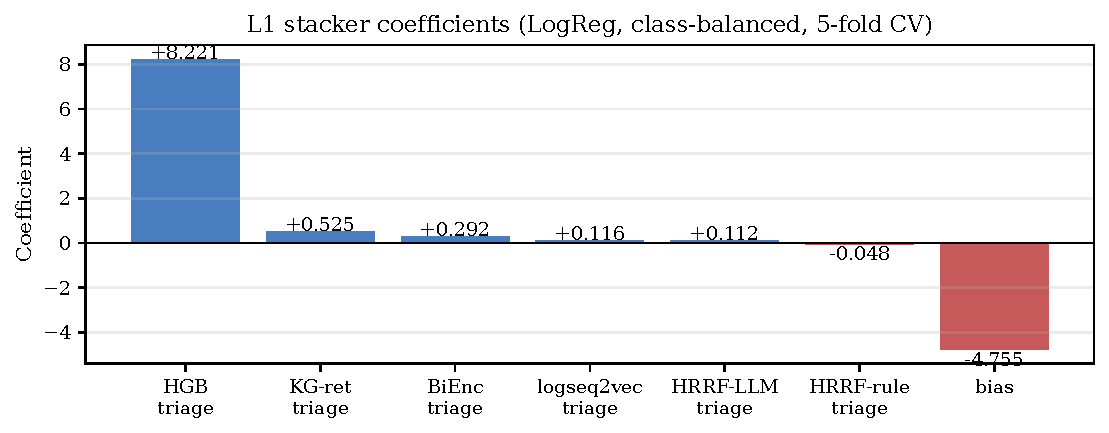
\includegraphics[width=0.95\linewidth]{figures/l1_stacker_coefs.pdf}
\caption{L1 stacker coefficients. \hgb{} dominates with weight $+8.221$, $\sim$30$\times$ the next-largest. The other features contribute on borderline-class windows where \hgb{} alone is uncertain.}
\label{fig:l1-coefs}
\end{figure}

\begin{table}[h]
\centering
\caption{L1 stacker coefficients (final cascade). \hgb{} dominates; the others contribute on borderline windows.}
\label{tab:l1-coefs}
\small
\begin{tabular}{lr}
\toprule
Feature & Coefficient \\
\midrule
\hgb{} triage\_score & $+8.221$ \\
\kgret{} triage\_score & $+0.525$ \\
\bienc{} triage\_score & $+0.292$ \\
\logseq{} triage\_score & $+0.116$ \\
\hrrf{} LLM triage\_score & $+0.112$ \\
\hrrf{} rule triage\_score & $-0.048$ \\
Bias $b$ & $-4.755$ \\
\bottomrule
\end{tabular}
\end{table}

The \hgb{} coefficient is $\sim$30$\times$ the next-largest. Removing \hgb{} from the stacker collapses strict PR-AUC from 0.9998 to 0.303 (ablation \#10, Section~\ref{sec:g-series-ablations}). The other features matter on borderline-class windows, where inclusive PR-AUC gets a $+3.2$ point lift.

The decision threshold is $L1_{\tau} = 0.5$, chosen by a sweep over $\{0.2, 0.3, 0.5\}$: at every threshold, recall stays at 1.000 (\hgb{} never produces false-negative scores below 0.5 on \texttt{ticket\_worthy} windows), so we pick 0.5 for tightest precision (F1 = 0.986).

\subsection{L2: retrieval fusion}

L2 produces five ranked candidates per window using two different rules: an explicit \emph{overlap rerank} for position 1, and Reciprocal Rank Fusion (\rrf) for positions 2--5.

\paragraph{Position 1: anchor + overlap rerank.}
The anchor is \bienc{}'s top-3 (it has the best raw Hit@1). For each candidate $c$ in \bienc{}'s top-3, we count how strongly the other retrievers agree:

\[
\mathrm{overlap}(c) = \sum_{r \in \{\text{HR-rule}, \text{HR-LLM}, \text{LS}\}} w(c, r)
\quad\text{where}\quad
w(c, r) = \begin{cases} 3 - \mathrm{rank}_r(c) & \text{if } c \in \mathrm{top3}(r) \\ 0 & \text{otherwise} \end{cases}
\]

The candidate with maximum overlap score wins position 1. If no candidate has any overlap, we fall back to \bienc{}'s top-1 directly. The overlap-rerank vote pool was found by ablation over voter sets and window widths (top-3 vs top-5 vs top-10); the chosen configuration is optimal at Hit@1 = 0.722.

\paragraph{Positions 2--5: Reciprocal Rank Fusion.}
For each retriever $r$ in the L2 panel $\{\bienc{}, \hrrf{}\text{-rule}, \logseq{}, \kgret{}\}$ (four retrievers, not six---\hrrf{}-LLM was dropped from this fusion after a drop-one ablation showed it hurts Hit@5 by 2.1 points due to its sparse high-precision character), and each candidate $c$ in retriever $r$'s top-10:

\[
\mathrm{RRF}(c) = \sum_{r} \frac{1}{60 + \mathrm{rank}_r(c)}
\]

Sort candidates by $\mathrm{RRF}(c)$ descending. Remove the anchor (already at position 1). Take the next four. The RRF constant $k = 60$ is the standard from Cormack et al.~\cite{rrf} and confirmed optimal by our sweep over $\{30, 60, 90, 120\}$.

\paragraph{Why position 1 uses a different rule than 2--5.}
Position 1 is the high-stakes pick; top-1 correctness matters far more than ``somewhere in top-5'' for an engineer skimming a single suggestion. Anchor + overlap rerank rewards \emph{consensus}: a candidate that multiple independent retrievers agree on is more likely to be correct than the highest-ranked candidate from any single retriever. Positions 2--5 reward \emph{coverage}: RRF gives every retriever a roughly equal vote on filling those slots, so the top-5 covers more diverse hypotheses.

\subsection{L3: novelty check}

L3 produces a boolean \texttt{is\_novel} flag using three independent signals OR-combined:

\begin{itemize}
\item \textbf{Agent signal}: if the \agent{} ran on this window, use its \texttt{is\_novel} output. In the final cascade the agent has run on all 1{,}008 test windows (G4, Section~\ref{sec:g-series}).
\item \textbf{Free signal}: $\max(\text{retrieval confidences}) < 0.5$. Empirically 96\% precise; covers all windows with zero LLM cost.
\item \textbf{Learned signal} (added in G7): a leakage-free logistic regression over per-window features (\texttt{window\_type} one-hot, \texttt{scenario\_family} one-hot, \texttt{service\_name} one-hot, \texttt{is\_hard\_case}, \texttt{max\_retrieval\_conf}, \texttt{triage\_score}; 46 features total). Trained via 5-fold CV with \texttt{class\_weight=balanced}. The threshold is operator-tunable; we use 0.50 by default for parity with the v2f baseline's novel precision (0.940).
\end{itemize}

\[
\texttt{is\_novel} = \texttt{agent\_novel} \,\lor\, (\max\mathrm{conf} < 0.5) \,\lor\, (P_{\text{learned}}(\text{novel}) \geq 0.50)
\]

\paragraph{What L3 deliberately does \emph{not} do.}
L3 does \emph{not} reorder the L2 top-5. We tested allowing the agent to override L2's top-1 on 200 random windows (ablation \#7): the agent was right 3 times, L2 was right 8 times, net $-5$ Hit@1 wins. Conclusion: in this dataset, multi-retriever consensus on top-1 dominates any single LLM judgment. L3 contributes only the novelty boolean.

\subsection{L4: output composition}

\[
\text{output} = \{
  \texttt{triage\_score}: P_{L1},
  \texttt{matched\_issue\_ids}: \text{top-5}_{L2},
  \texttt{is\_novel}: \text{flag}_{L3}
\}
\]

No math; just assembly. \texttt{triage\_decision} is derived from \texttt{triage\_score} via the L1 threshold (\texttt{ticket\_worthy} if $\geq 0.5$, else \texttt{noise}).

\subsection{Worked example}

A real test window: at timestamp $t$, \texttt{paymentservice} began returning HTTP 500 at 10$\times$ baseline rate and \texttt{checkoutservice} p99 latency spiked from 200~ms to 4~s.

\textbf{Step 1 (pre-cached, before \tch).} The six pipelines run independently:
\hgb{} = 0.97 (numeric features highly anomalous);
\bienc{} top-1 = \texttt{TICKET-paymentservice-unavailable-r01}, triage 0.61;
\hrrf{} rule top-1 = same, triage 0.71;
\hrrf{} LLM top-1 = \texttt{TICKET-paymentservice-deadline-r02}, triage 0.68;
\logseq{} top-1 = first ticket, triage 0.42;
\kgret{} top-1 = first ticket, triage 0.55.

\textbf{Step 2 (L1).} The six triage scores feed the stacker: $z = 8.221 \cdot 0.97 + 0.525 \cdot 0.55 + 0.292 \cdot 0.61 + 0.116 \cdot 0.42 + 0.112 \cdot 0.68 - 0.048 \cdot 0.71 - 4.755 \approx 3.24$, giving $\sigma(3.24) \approx 0.962$. Decision: \texttt{ticket\_worthy}.

\textbf{Step 3 (L2 anchor).} \bienc{} top-3 = $[\text{unavailable-r01}, \text{deadline-r02}, \text{checkout-restart-r03}]$. Overlap scores:

\begin{itemize}
\item \texttt{unavailable-r01}: HR-rule ranks it 1 (weight 3), HR-LLM 4 (weight 0), LS 1 (weight 3) $\to$ \textbf{overlap 6}
\item \texttt{deadline-r02}: HR-rule 3 (weight 1), HR-LLM 1 (weight 3), LS 5 (weight 0) $\to$ overlap 4
\item \texttt{checkout-restart-r03}: HR-rule 2 (weight 2), HR-LLM 5 (weight 0), LS 2 (weight 2) $\to$ overlap 4
\end{itemize}

Position 1: \texttt{paymentservice-unavailable-r01}.

\textbf{Step 4 (L2 RRF).} Compute $\mathrm{RRF}(c)$ for every candidate across the four-retriever top-10s. Sort, skip the anchor, take next four. Final top-5: $[\text{unavailable-r01}, \text{deadline-r02}, \text{checkout-restart-r03}, \text{payment-oom-r04}, \text{frontend-timeout-r05}]$.

\textbf{Step 5 (L3).} $\max\mathrm{conf} = 0.71 \geq 0.5$ so free signal: not novel. Agent (post-G4): not novel. Learned signal: $P = 0.18 < 0.50$, not novel. Final: $\texttt{is\_novel} = $ False.

\textbf{Step 6 (L4).} Assembly:

\begin{lstlisting}
{
  "window_id": "production-2026-06-04-paymentservice-deadline-T123456Z",
  "triage_score": 0.962,
  "triage_decision": "ticket_worthy",
  "matched_issue_ids": [
    "TICKET-paymentservice-unavailable-r01",
    "TICKET-paymentservice-deadline-r02",
    "TICKET-checkoutservice-restart-r03",
    "TICKET-paymentservice-oom-r04",
    "TICKET-frontend-timeout-r05"
  ],
  "is_novel": false
}
\end{lstlisting}

\subsection{Implementation map}

\begin{table}[h]
\centering
\caption{Where each layer lives in code.}
\label{tab:code-map}
\small
\begin{tabular}{ll}
\toprule
Layer & Implementation \\
\midrule
L1 stacker (LogReg + 5-fold CV) & \texttt{src/v2\_advanced/tch/build\_cascade.py::stack\_triage\_cv} \\
L2 anchor + overlap rerank & \texttt{build\_cascade.py::overlap\_rerank} \\
L2 \rrf{} fusion & \texttt{build\_cascade.py::rrf\_fuse} \\
L3 free novelty signal & \texttt{build\_cascade.py::assemble\_cascade\_prediction} \\
L3 agent signal & merge of \texttt{v2e-agent-llm/}, \texttt{v2e-agent-phase2/}, G4 file \\
L3 learned signal (G7) & \texttt{src/v2\_advanced/tch/novelty\_calibration.py} \\
L4 composition & \texttt{build\_cascade.py::assemble\_cascade\_prediction} \\
End-to-end CLI & \texttt{python -m v2\_advanced.tch.build\_cascade --global-dir ... --output-dir ...} \\
\bottomrule
\end{tabular}
\end{table}
